% This is samplepaper.tex, a sample chapter demonstrating the
% LLNCS macro package for Springer Computer Science proceedings;
% Version 2.21 of 2022/01/12
%
\documentclass[runningheads]{llncs}
%
\usepackage[T1]{fontenc}
% T1 fonts will be used to generate the final print and online PDFs,
% so please use T1 fonts in your manuscript whenever possible.
% Other font encondings may result in incorrect characters.
%
\usepackage{graphicx}
\usepackage{booktabs}
\usepackage{tabularx}
\usepackage{makecell}
\usepackage{multirow}
\usepackage{array}
\usepackage{amsmath}
\usepackage{amsfonts}
\usepackage{amssymb}
\usepackage{amsmath}
\usepackage{hyperref} 
\usepackage{algorithm}
\usepackage{algpseudocode}
% Used for displaying a sample figure. If possible, figure files should
% be included in EPS format.
%
% If you use the hyperref package, please uncomment the following two lines
% to display URLs in blue roman font according to Springer's eBook style:
\usepackage{color}
\renewcommand\UrlFont{\color{blue}\rmfamily}
\urlstyle{rm}
%
\begin{document}
	
	\title{Basis-Guided Counterfactual Generation for Explainable Multivariate Time Series Models}
	
	%\titlerunning{Underwater Basket Weaving Under Extreme Pressure}
	% If the full title of your paper is short enough to also fit in the running head, you can omit the abbreviated paper title here. You can check as follows: if you comment out the \titlerunning line, something will appear in the header of all odd-numbered pages of your PDF from page 3 onward. This something is either the full title (in which case all is well), or the error message "Title Suppressed Due to Excessive Length". If this error message appears, you're going to want to provide an abbreviated title within the \titlerunning command, because if you won't do it, Springer will do it for you.
	
	%N.B.: Author information (both in the \author{} and \authorrunning{} command) should only be present in the Camera-Ready Version of your paper. The version that you initially submit for review, ought to be double-blind. So, when initially submitting your paper, use:
	
	
%	\author{Author information scrubbed for double-blind reviewing}
%	\author{Nirban Das\inst{1}\orcidID{0009-0008-5907-9397} \and 
%		Vaibhav Rajanand Wankar\inst{1} \and
%		Rashmi Dutta Baruah\inst{1}\orcidID{0000-0002-6756-8157} 
%		% \corr \and Antwan Andr\'e Patton\inst{1}\orcidID{0000-1111-2222-3333}
%	}
%	
%	
%	\institute{Indian Institute of Technology Guwahati, India \email{\{d.nirban,w.vaibhav,r.duttabaruah\}@fiitg.ac.in}
%		%\and Secondary European Affiliation, Tiergartenstr. 17, 69121 Heidelberg, Germany\email{lncs@springer.com}
%	}
	
	
	\maketitle              % typeset the header of the contribution
	
	\begin{abstract}
		Explainability in time series is critical for establishing trust in deep learning models. While counterfactual explanations offer a path to understanding model decisions by suggesting minimal changes to input data, that is, "what would need to change for the model to predict a different outcome", existing approaches often treat time-series data as independent features and optimise the perturbations directly over it. In the case of multivariate sensor data, this often yields jittery, high-frequency changes that can satisfy the model, but the counterfactuals generated physically might not be plausible. To address this, we propose a novel method that parameterises counterfactual perturbations using smooth temporal basis functions (e.g., B-Splines, Fourier) rather than raw time steps. By optimising weights in a low-dimensional basis space, it inherently enforces temporal coherence, eliminating unrealistic noise without requiring complex physics-based constraints. We further introduce a diversity mechanism based on Determinantal Point Processes (DPPs) in the coefficient space to generate distinct, valid counterfactual trajectories. To evaluate the proposed method, we used various multivariate time series datasets and generated counterfactuals. We compared our proposed approach with the state-of-the-art methods; our approach consistently produces valid counterfactuals while achieving a better trade-off between proximity, sparsity, and temporal smoothness than existing baselines.
		
		\keywords{Explainable AI \and Basis Functions \and Counterfactual Explanation \and Multivariate Time Series.}
	\end{abstract}
	
	\section{Introduction}
	With recent advancement in Machine Learning, we see that deep learning models perform good and had become a standard for complex prediction tasks. While these models being adopted and deployed in the high-stake domains these models lacks limited interpretability and explianability\cite{WILKINSON2026200647}. This lack of transparency is risky in high-stakes settings like healthcare, industrial monitoring, finance, and autonomous decision support, where interpretability is closely tied to trust, accountability, and safe adoption. Recent reviews of Explainable Artificial Intelligence (XAI) continue to identify explanation quality, robustness, and evaluation as open challenges for real-world deployment\cite{LONGO2024102301,MOHAMED2025200595}.
	
	A large part of the XAI literature has focused on feature-attribution and local surrogate methods\cite{XAI_Core_Sol_ACM_10.1145/3561048}, such as LIME\cite{LIME_10.1145/2939672.2939778} and SHAP\cite{SHAP_10.5555/3295222.3295230}, which explain predictions by estimating the contribution of input variables. These methods are useful for highlighting which parts of an input were influential (feature importance) and for explaining \textit{why} the model predicted a given outcome and which feature contributed the most. But, these models do not show \textit{How} the outcome could be changed. This can be tackled using counterfactual explanations, which provide alternative inputs that are close to the original instance yet lead to the desired prediction. Since the influential work of Wachter et al. \cite{wachter2017counterfactual}, counterfactual explanations have become a prominent paradigm because they are naturally aligned with recourse, intervention, and actionability.
	
	Despite rapid progress, most counterfactual methods were originally developed for tabular data \cite{CF_LIT_Rev_10.1007/s10618-022-00831-6}. The time-series setting is considerably more difficult because sequential data exhibit temporal dependence, local continuity \cite{Learn_CF_Intervals_10.1145/3627673.3679952}, and, in multivariate settings, strong cross-channel interactions. These methods, naively perturb individual time points may flip the model output while producing unrealistic, noisy, or physically implausible trajectories. This limitation has been repeatedly noted in the emerging literature on XAI for time series, which remains far less mature than its tabular counterpart. Early and recent methods such as Glacier \cite{Wang2024} have demonstrated the promise of time-series-specific counterfactual generation, but they also highlight the difficulty of balancing validity, sparsity, and temporal coherence.
	
	In this paper we propose our novel approach to generate Counterfactuals for multivariate time series through a temporal basis formulation. Instead of optimising unrestricted perturbations over raw time steps, the proposed method parameterises counterfactual changes in a low-dimensional basis space using smooth temporal basis functions such as B-splines or Fourier bases. This embeds temporal coherence directly into the search space and helps generate explanations that are not only valid and proximal, but also smoother, more plausible, and easier to interpret as realistic alternative trajectories. In addition, diversity is encouraged in the coefficient space to produce multiple non-redundant counterfactual explanations for the same query instance.
	
	\section{Related Work}
	
	Most explainability methods are post-hoc, where we do not open the black box. Local Interpretable Model-agnostic Explanations (LIME) \cite{LIME_10.1145/2939672.2939778} explains an individual prediction by sampling perturbations around the instance and fitting an interpretable model locally, giving a faithful-but-local approximation of the decision surface. SHapley Additive exPlanations (SHAP) \cite{SHAP_10.5555/3295222.3295230} provides an explanation from a game theoretic approach by assigning each feature an importance value for a particular prediction by the black-box model. When explaining models trained on time series data using a tabular approach, they can generate out-of-distribution subsequences and ignore temporal dependence \cite{hase2021out}. This has motivated the development of various explainability methods explicitly for time series scenarios, such as TimeSHAP \cite{bento2021timeshap}, which uses sequence perturbations, and KernelSHAP \cite{SHAP_10.5555/3295222.3295230}, which extends KernelSHAP to sequential data to explain Recurrent Neural Networks (RNNs). TIMING \cite{jang2025timing} uses conventional Integrated Gradients (IG) \cite{Integrated_Grad_10.5555/3305890.3306024} for feature attributions. 
	
	Counterfactual explanations are one of the most important topics in the field of explainable AI because they move beyond descriptive importance scores and instead provide actionable explanations: they indicate how an input would need to change in order to obtain a different prediction. This has deep roots from Structural Causal Models(SCM) by Judea Pearl, which formalises counterfactual queries via interventions and structural equations, setting a principled foundation for "what-if" reasoning\cite{CF_Pearl_10.1093/logcom/exm048}. In \cite{wachter2017counterfactual}, Wachter et al. popularised counterfactual explanations (CFEs) for black-box automated decisions by framing them as minimal changes that would flip an outcome without exposing model internals. In \cite{DiCE_Mothilal_2020} DiCE was introduced where CFEs are generated are diverse as it used determinantal point processes (DPP) objective.
	
	Although counterfactual explanation is now well developed for tabular data, the time-series setting remains much less mature. This is mainly because sequential data introduce temporal dependence, high dimensionality, and strong structural constraints: changing isolated values may flip a prediction while producing unrealistic trajectories. In \cite{delaney2021instance} the authors proposed "Native Guide" that generates CFEs by adapting discriminative regions toward a target-class guide. Glacier \cite{wang2024glacier}, a model-agnostic method designed specifically for generating locally-constrained counterfactual explanations for univariate time series classification, leveraging gradient search in either the original or a latent space learned via an auto-encoder. In \cite{bahri2024discord} DiscoX, a Discord-based Counterfactual Explanation algorithm, as a post-hoc, model-agnostic method for time series classification models. In \cite{Sub-SpaCE_10.1007/978-3-031-63800-8_1}Sub-SpaCE uses a genetic algorithm to enforce sparsity and contiguity via subsequence edits. forecasting CFEs were explicitly formulated in ForecastCF\cite{wang2023counterfactual}, and the input data is gradually adjusted a little at a time using gradient-based optimisation. In \cite{CoMTE_9462056}, CoMTE was introduced, where the CFEs were generated for multivariate time series data by finding similar examples from the training set that already give the desired output, and it then swaps a small number of variables from those examples into the current samples until the prediction changes.

    % For multivariate time series scenarios in \cite{shapeletbasedcounterfactualexplanationsmultivariate}, it develops a model-agnostic CFE algorithm by leveraging the inherent interpretability of shapelets. In \cite{huang2024shapelet} Proposes Time-CF, a model-agnostic, instance-based, post-hoc explainability method that leverages shapelets and TimeGAN to generate counterfactual explanations for time series classifiers.
    
	To summarize the existing methodologies, we can see that most of the CFE generation methods performs well and uses various techniques like, nearest-neighbour, optimization in the latent space. Generating multivariate Counterfactuals is challenging, as preserving inter-channel correlation and temporal smoothness while ensuring validity and sparsity is difficult. Therefore, we generate our CFE on a smooth basis, which yields a non-redundant solution.
	
	\section{Methodology}
	
	Let the input be a time-series instance $\mathbf{X} \in \mathbb{R}^{T \times D}$, where $T \in \mathbb{N}$ is the sequence length and $D$ is the number of sensor features. The input instance $X \in \mathbf{R}^{T \times D}$ be the query instance(the original time series data) for which we seek an explanation for the data be, 
	
	\begin{equation}
		\mathbf{X} = [\mathbf{x}_1, \mathbf{x}_2, \dots, \mathbf{x}_T]^\top, \quad \text{where } \mathbf{x}_t \in \mathbb{R}^{D}, t \in \{1,2,...T\}
	\end{equation}
	
	We train a predictive model like Transformer or LSTM, let it be 
	
	\begin{equation}
		\label{eq:trained_model}
		f: \mathbb{R}^{T \times D} \to \mathbb{R}
	\end{equation}
	
	We train the model as defined in Equation \ref{eq:trained_model} to predict the $\hat{y}$ for example RUL(remaining Useful Life) of a machine/engine  
	\begin{equation}
		\label{eq:RUL}
		\hat{y} = f(\mathbf{X}) \in \mathbb{R}^+
	\end{equation}
	
	\subsection{Counterfactual Explanations}
	Counterfactual explanations answer the question: "What is the minimal change to the input features that would result in a desired different outcome?" In our context, this translates to: "What are the smallest changes in the sensor reading history that would result in the RUL prediction falling within a desired range?". We seek a counterfactual instance $\mathbf{X_{cf}}$ such that $ f(\mathbf{X_{cf}}) \approx y_{target}$, where $y_{target}$ is the Target value we want to achieve by the model $f$, for that we would do a minimal change to the original $\mathbf{X}$ 
	
	\begin{equation}
		\label{eq:cf_basic}
		\mathbf{X_{cf}} = \mathbf{X} + \mathbf{\Delta}
		\quad \text{where } \mathbf{\Delta} \in \mathbb{R}^{T \times D}
	\end{equation}
	
	From Equation \ref{eq:cf_basic} we define $\mathbf{\Delta}$ as a free parameter matrix, the $\mathbf{\Delta}$ is constrasined to lie in the span of a smooth basis $\mathbf{\Phi}$, $\mathcal{B} = \{ \phi_k \}_{k=1}^K$ be a set of $K$ distinct temporal basis functions, where $K \ll T$. and construct the Basis Projection Matrix $\mathbf{\Phi} \in \mathbb{R}^{T \times K}$
	
	\begin{equation}
		\mathbf{\Phi} = 
		\begin{bmatrix}
			\phi_1(1) & \phi_2(1) & \dots & \phi_K(1) \\
			\phi_1(2) & \phi_2(2) & \dots & \phi_K(2) \\
			\vdots & \vdots & \ddots & \vdots \\
			\phi_1(T) & \phi_2(T) & \dots & \phi_K(T)
		\end{bmatrix}
	\end{equation}
	
	We define a learnable weight matrix $\mathbf{W} \in \mathbb{R}^{K \times D}$ such that for a $w_{k,m}$ it represents the contribution of the basis function $k$ to sensor $m$. The pertubations $\mathbf{\Delta}(\mathbf{W})$ is defined by the linear projection.
	
	\begin{equation}
		\label{eq:lin_proj}
		\mathbf{\Delta}(\mathbf{W}) = \mathbf{\Phi}\mathbf{W}
	\end{equation}
	
	So From Equation \ref{eq:cf_basic} and Equation \ref{eq:lin_proj} the counterfactual parameterized by $\mathbf{W}$ is 
	
	
	\begin{equation}
		\label{eq:xcf_schema}
		\mathbf{X}_{\mathrm{cf}} = \Pi_{\mathcal{S}}(\mathbf{X} + \mathbf{\Phi}\mathbf{W}).
	\end{equation}
	
	The operator \(\Pi_{\mathcal{S}}\) strictly enforces mutability masks (preventing edits on immutable or contextual features), feature-wise minimum and maximum bounds, and static-feature consistency over time.
	The feature schema ($\mathcal{S}$) serves as a rigorous specification of domain knowledge and physical constraints for the multivariate time series.
	It explicitly defines the role of each variable, distinguishing between actionable features that can be modified and those that are strictly immutable.
	
	To generate a diverse set of \(N\) counterfactuals for a single query, we jointly optimise a collection of coefficient matrices \(\mathcal{W}=\{\mathbf{W}^{(1)},\dots,\mathbf{W}^{(N)}\}\). The overall loss function \(\mathcal{J}(\mathcal{W})\) balances predictive validity with several competing regularisation terms to ensure plausibility:
	\begin{equation}
		\label{eq:total_loss}
		\mathcal{J}(\mathcal{W}) = \lambda_v \mathcal{L}_{\mathrm{valid}} + \rho \mathcal{L}_{\mathrm{valid}}^2 + \rho \left( \mathcal{L}_{\mathrm{cleanup}} \right),
	\end{equation}
	where \(\rho > 0\) is a dynamic augmented penalty coefficient that grows if the optimization stagnates, and \(c\) is a binary or fractional scaling factor used to down-weight the cleanup terms until the search discovers an initially valid region. The cleanup objective is defined as:
	\begin{equation}
		\label{eq:cleanup_loss}
		\mathcal{L}_{\mathrm{cleanup}} = \lambda_p \mathcal{L}_{\mathrm{prox}} + \lambda_c \mathcal{L}_{\mathrm{coef}} + \lambda_g \mathcal{L}_{\mathrm{group}} + \lambda_s \mathcal{L}_{\mathrm{smooth}} + \lambda_d \mathcal{L}_{\mathrm{div}} + \lambda_{\mathrm{sl}} \mathcal{L}_{\mathrm{state}}.
	\end{equation}
	
	
	%	To generate a set of $N$ diverse counterfactuals we optimize on the weights $\mathcal{W} = \{ \mathbf{W}^{(1)}, \dots, \mathbf{W}^{(N)} \}$ such that our total loss is :
	%	
	%	\begin{equation}
		%		\label{eq:cf_total_loss}
		%		\begin{split}
			%			\mathcal{J}(\mathcal{W}) ={}& \lambda_v \mathcal{L}_{\mathrm{valid}}
			%			+\rho\,\mathcal{L}_{\mathrm{valid}}^{2} \\
			%			& +c\left(
			%			\lambda_p\mathcal{L}_{\mathrm{prox}} 
			%			+\lambda_c\mathcal{L}_{\mathrm{coef}}
			%			+\lambda_g\mathcal{L}_{\mathrm{group}}
			%			+\lambda_s\mathcal{L}_{\mathrm{smooth}}
			%			+\lambda_d\mathcal{L}_{\mathrm{div}}
			%			\right)
			%		\end{split}
		%	\end{equation}
	
	The \textbf{Validity} Loss $\mathcal{L}_{\text{valid}}$ ensures that the counterfactuals generated achieve the desired prediction. For a regression task, the target output can be set to  an interval of $y_{target} \in[y_{min}, y_{max}]$
	\begin{equation}
		\label{eq:cf_L_validity}
		\mathcal{L}_{\text{valid}} = \frac{1}{N} \sum_{i=1}^N \left( max(0,y_{min} - f(\mathbf{X}_{cf}))^2 + max(0, f(\mathbf{X}_{cf}) - y_{max})^2 \right)
	\end{equation}
	
	The \textbf{Proximity} Loss ($\mathcal{L}_{\text{prox}}$) is to penalise large deviations from the original input, encouraging minimal, actionable changes. To achieve this, we use our proximity loss, similar to that of Wachter \cite{wachter2017counterfactual}. so for each feature d in $D$, the $m_{d}^{-1}$ is generally set to $1$ 
	
	\begin{equation}
		med_d = median_j(x_{j, d}),
		\quad MAD_d = median_j(|x_{j,d} -med_d|)
	\end{equation}
	
	\begin{equation}
		\label{eq:MAD}
		m_{d}^{-1} = \frac{1}{MAD_d + \epsilon} 
	\end{equation}
	
	From Equation \ref{eq:MAD} the Proximity Loss is
	
	\begin{equation}
		\label{eq:L_prox}
		\mathcal{L}_{\text{prox}} = \frac{1}{N} \sum_{i = 1}^{N} \left\| \mathbf{\Phi}\mathbf{W}^{(i)} m_{d}^{-1} \right\|_F^{2}
	\end{equation}
	
	The \textbf{Coefficient Sparsity} Loss ($\mathcal{L}_{\text{coef}}$) encourages compact counterfactual explanations in
	the basis space, we penalise the $\ell_1$-norm of the basis coefficients. 
	
	\begin{equation}
		\label{eq:cf_L_sparse}
		\mathcal{L}_{\text{coef}} = \frac{1}{N} \sum_{i = 1}^{N} \left\| \mathbf{W}^{(i)} \right\|_1
	\end{equation}
	
	Rather than applying pointwise sparsity in the time domain, we apply a Group Lasso penalty across predefined sets of actionable features $\mathcal{G}=\{g_1,\dots,g_M\}$. The \textbf{Channel Group Sparsity} ($\mathcal{L}_{\mathrm{group}}$) ensures the explanation acts on the smallest necessary number of distinct sensor channels:
	
	\begin{equation}
		\label{eq:group_sparsity}
		\mathcal{L}_{\mathrm{group}} = \frac{1}{N} \sum_{i=1}^{N} \sum_{g \in \mathcal{G}} \sqrt{ \sum_{t=1}^{T} \sum_{d \in g} (\Delta_{t,d}^{(i)})^2 }.
	\end{equation}
	
	The \textbf{Smoothness} Loss ($\mathcal{L}_{\text{smooth}}$) regularises temporal irregularities; it penalises rapid and sudden temporal changes in the counterfactual perturbation in Equation \ref{eq:lin_proj} by measuring its discrete curvature (second difference) over time. Concretely, for each counterfactual $i$ and feature $d$, $\mathbf{\Delta}^{(i)} = \mathbf{\Phi}\mathbf{W}^{(i)}$, then the second order derivative of $\mathbf{\Delta}$ also known as the Roughness Penalty \cite{green1993nonparametric}. 
	
	\begin{equation}
		\mathbf{\nabla}^2(\mathbf{\Delta}^{(i)})_{t, d} = \mathbf{\Delta}^{(i)}_{t+1, d} -2\mathbf{\Delta}^{(i)}_{t, d} + \mathbf{\Delta}^{(i)}_{t-1, d}
	\end{equation}
	
	\begin{equation}
		\mathcal{L}_{\text{smooth}}(\mathcal{W}) = \frac{1}{N(T-2)D} \sum_{i=1}^{N}\sum_{t=2}^{T-1}\sum_{2=1}^{D} (\mathbf{\Delta}^{(i)}_{t+1, d} -2\mathbf{\Delta}^{(i)}_{t, d} + \mathbf{\Delta}^{(i)}_{t-1, d})^2
	\end{equation}
	
	The \textbf{Diversity} Loss via Determinantal Point Processes(DPP) ($\mathcal{L}_{\text{dpp}}$) is to shape diverse trajectories of $N$ counterfactuals. DPP ensures that the set of counterfactuals is non-redundant \cite{Kulesza_2012} \cite{DiCE_Mothilal_2020}.
	
	\begin{equation}
		\hat{\mathbf{v}}_i = \frac{\text{vec}(\mathbf{W}^{(i)})}{\left\| \text{vec}(\mathbf{W}^{(i)}) \right\|_{2}} 
	\end{equation}
	
	\begin{equation}
		S_{i,j} = {\hat{\mathbf{v}}_i}^T \hat{\mathbf{v}}_i
	\end{equation}
	
	\begin{equation}
		\mathcal{L}_{\text{dpp}}(\mathcal{W}) = - log(det(\mathbf{S} + \epsilon \mathbf{I}))
	\end{equation}
	
	In real-world time series, actionable recourse should ideally target manipulable \textit{action} features rather than endogenous \textit{state} variables. To prevent optimisation infeasibility while still discouraging state alterations, our feature schema $\mathcal{S}$ applies a soft $\ell_1$-norm penalty, the State Lock Loss ($\mathcal{L}_{\mathrm{state}}$), to perturbations strictly within the state-feature subset $\mathcal{D}_{\mathrm{state}} \subseteq \{1, \dots, D\}$
	
	\begin{equation}
		\label{eq:state_lock_loss}
		\mathcal{L}_{\mathrm{state}} = \frac{1}{NT|\mathcal{D}_{\mathrm{state}}|} \sum_{i=1}^{N} \sum_{t=1}^{T} \sum_{d \in \mathcal{D}_{\mathrm{state}}} \left| \Delta_{t,d}^{(i)} \right|.
	\end{equation}
	By incorporating this term into the overall cleanup objective with a weight $\lambda_{\mathrm{sl}}$, the optimization framework is encouraged to prioritize recourse through actionable channels, resorting to state modifications only when strictly necessary to cross the target decision boundary.
	
	
	%	The \textbf{State Lock Loss} ($\mathcal{L}_{\text{state}}$) term softly discourages changes on state features. In practice, it is included only when state-lock regularisation is enabled. Let $\mathcal{D}_{\mathrm{state}}\subseteq\{1,\dots,D\}$ denote the set of state-feature indices. The optional state-lock regulariser is defined as:
	%	
	%	\begin{equation}
		%		\label{eq:state_lock_loss_final}
		%		\mathcal{L}_{\mathrm{state}} = \frac{1}{NT|\mathcal{D}_{\mathrm{state}}|}
		%		\sum_{i=1}^{N}\sum_{t=1}^{T}\sum_{d \in \mathcal{D}_{\mathrm{state}}}
		%		\left|
		%		\Delta_{t,d}^{(i)}
		%		\right|.
		%	\end{equation}
	
	%	to find a counterfactual instance $\mathbf{X_{cf}}$ that minimizes a loss function, $\mathcal{J}(\mathcal{W})$, balancing five competing objectives:
	%	
	%	\begin{equation}
		%		\label{eq:cf_opt_obj}
		%		\begin{aligned}
			%			\mathbf{X}^* = \arg\min_{X_{cf}} \mathcal{J}(\mathcal{W}) 
			%		\end{aligned}
		%	\end{equation}
	
	Thus, the overall optimisation problem seamlessly balances validity, continuous schema constraints, and temporal plausibility in the basis space:
	\begin{equation}
		\label{eq:cf_optimisation_problem_final}
		\mathcal{W}^{*}
		=
		\arg\min_{\mathcal{W}} \mathcal{J}(\mathcal{W}),
		\qquad
		\mathbf{X}_{\mathrm{cf}}^{(i)*}
		=
		\Pi_{\mathcal{S}}\!\left(\mathbf{X}+\mathbf{\Phi}\mathbf{W}^{(i)*}\right),
		\quad i=1,\dots,N.
	\end{equation}
	
	Our Algorithm \ref{alg:basis_cf} generates counterfactual time series by optimising a low-dimentional coefficient tensor $\mathbf{W}$ insted of perturbating each time step independently. For any chosen Basis family we first construct a temporal basis matrix $\mathbf{\Phi}$, then we project the $\mathbf{W}$ into the input space $\mathbf{\Delta} = \mathbf{\Phi W}$, next we form the candidate counterfactuals as $\mathbf{X_{cf}} = \Pi_{\mathcal{S}}(\mathbf{X} + \mathbf{\Delta})$, where $\Pi_{\mathcal{S}}$ enforces mutability masks, bounds, and optional structural constraints. The optimisation objective combines a validity term with proximity, coefficient sparsity, group/channel sparsity, smoothness, and diversity penalties; we implement the validity as an augmented-penalty style through $\lambda_v \mathcal{L}_{\mathrm{valid}}
	+\rho\,\mathcal{L}_{\mathrm{valid}}^{2}$. The optimisation is performed over multiple restarts, using Adam \cite{2015-kingma} for the main search and optional LBFGS\cite{liu1989limited} refinement, and the final counterfactual set is selected by a validity-first lexicographic criterion: valid solutions are preferred first, and ties are broken by validity error, proximity, group sparsity, and smoothness.
	
	\begin{algorithm}[H]
		\caption{Basis-Guided Counterfactual Generation}
		\label{alg:basis_cf}
		\begin{algorithmic}[1]
			\Require Predictor $f$, query $\mathbf{X} \in \mathbb{R}^{T \times D}$, target $\mathcal{T}$, schema $\mathcal{S}$, basis $\mathbf{\Phi}$, CF count $N$.
			\Ensure Optimal counterfactual set $\mathbf{X}_{\mathrm{cf}}^{\star}$.
			
			\State Init global best $K_{\mathrm{global}} \gets (\infty, \dots, \infty)$, $\mathbf{X}_{\mathrm{cf}}^{\star} \gets \text{null}$, construct $\mathbf{\Phi}$.
			
			\For{restart $r = 1 \dots R$}
			\State Init $\mathbf{W}$ (zeros if $r=1$, else $\mathcal{N}(0, \sigma_{\mathrm{init}})$ shifted by previous best).
			\State $\rho \gets \rho_{\mathrm{init}}$, $p \gets 0$, $K_{\mathrm{local}} \gets (\infty, \dots, \infty)$, $\text{ever\_valid} \gets \text{False}$.
			
			\For{step $s = 1 \dots S_{\mathrm{Adam}}$} \Comment{\textbf{Phase 1: Adam Search}}
			\State $c \gets 1.0$ if $\text{ever\_valid}$ else $c_{\mathrm{prevalid}}$
			\State $\mathbf{X}_{\mathrm{cf}}, \mathbf{\Delta} \gets \Pi_{\mathcal{S}}(\mathbf{X} + \mathbf{\Phi}\mathbf{W})$ \Comment{Continuous schema constraints}
			\State $\mathcal{J} \gets \lambda_v \mathcal{L}_{\mathrm{valid}}(f(\mathbf{X}_{\mathrm{cf}})) + \rho \mathcal{L}_{\mathrm{valid}}^2 + c \mathcal{L}_{\mathrm{cleanup}}$
			\State Update $\mathbf{W}$ via Adam step minimizing $\mathcal{J}$.
			
			\State $K \gets (\text{invalid}, \mathcal{L}_{\mathrm{valid}}, \mathcal{L}_{\mathrm{prox}}, \mathcal{L}_{\mathrm{group}}, \mathcal{L}_{\mathrm{smooth}})$
			\State \textbf{if} $K < K_{\mathrm{local}}$ \textbf{then} $K_{\mathrm{local}} \gets K$, $\mathbf{W}_{\mathrm{local}}^{\star} \gets \mathbf{W}$, $p \gets 0$ \textbf{else} $p \gets p + 1$
			\State \textbf{if} $\max(\text{violation}) \le \epsilon$ \textbf{then} $\text{ever\_valid} \gets \text{True}$
			\State \textbf{if} $\neg \text{ever\_valid}$ and $s \bmod 25 == 0$ \textbf{then} $\rho \gets \min(\rho \cdot \rho_{\mathrm{growth}}, \rho_{\mathrm{max}})$
			\State \textbf{if} $\text{ever\_valid}$ and $p \ge p_{\mathrm{max\_patience}}$ \textbf{then break}
			\EndFor
			
			\If{$S_{\mathrm{LBFGS}} > 0$} \Comment{\textbf{Phase 2: L-BFGS Refinement}}
			\State Refine $\mathbf{W}_{\mathrm{local}}^{\star}$ via L-BFGS; update $K_{\mathrm{local}}, \mathbf{W}_{\mathrm{local}}^{\star}$ if improved.
			\EndIf
			
			\State $\mathbf{X}_{\mathrm{cf}}^{\mathrm{final}} \gets \Pi_{\mathcal{S}}^{\mathrm{final}}(\mathbf{X} + \mathbf{\Phi}\mathbf{W}_{\mathrm{local}}^{\star})$ \Comment{Final discrete constraints}
			\State \textbf{if} $K_{\mathrm{local}} < K_{\mathrm{global}}$ \textbf{then} $K_{\mathrm{global}} \gets K_{\mathrm{local}}$, $\mathbf{X}_{\mathrm{cf}}^{\star} \gets \mathbf{X}_{\mathrm{cf}}^{\mathrm{final}}$
			\EndFor
			
			\State \Return $\mathbf{X}_{\mathrm{cf}}^{\star}$
		\end{algorithmic}
	\end{algorithm}
	
	%	\begin{algorithm}[H]
		%		\caption{Basis-Guided Counterfactual Generation}
		%		\label{alg:basis_cf}
		%		\begin{algorithmic}[1]
			%			\Require 
			%			Trained predictor $f$, query sequence $\mathbf{X} \in \mathbb{R}^{T \times D}$, target specification $\mathcal{T}$, 
			%			feature schema $\mathcal{S}$, temporal basis matrix $\mathbf{\Phi} \in \mathbb{R}^{T \times K}$, number of CFs $N$.
			%			\Ensure 
			%			Optimal counterfactual set $\mathbf{X}_{\mathrm{cf}}^{\star}$.
			%			
			%			\State Construct basis matrix $\mathbf{\Phi}$ according to the selected basis family.
			%			\State Initialize global best key $K_{\mathrm{global}} \gets (\infty, \infty, \infty, \infty, \infty)$.
			%			\State Initialize global best counterfactual $\mathbf{X}_{\mathrm{cf}}^{\star} \gets \text{null}$.
			%			
			%			\For{restart $r = 1, \dots, R$}
			%			\If{$r = 1$}
			%			\State Initialize coefficients $\mathbf{W} \gets \mathbf{0} \in \mathbb{R}^{N \times K \times D}$
			%			\Else
			%			\State Initialize $\mathbf{W} \sim \mathcal{N}(0, \sigma_{\mathrm{init}})$ (optionally shifted by previous best $\mathbf{W}$)
			%			\EndIf
			%			
			%			\State Set $\rho \gets \rho_{\mathrm{init}}$, $p \gets 0$ (patience), $\text{ever\_valid} \gets \text{False}$.
			%			\State Initialize local best key $K_{\mathrm{local}} \gets (\infty, \dots, \infty)$.
			%			
			%			\State \textbf{// Phase 1: Exploratory Search (Adam)}
			%			\For{step $s = 1, \dots, S_{\mathrm{Adam}}$}
			%			\State $c \gets 1.0$ if $\text{ever\_valid}$ else $c_{\mathrm{prevalid}}$ \Comment{Down-weight cleanup before valid}
			%			\State $\mathbf{\Delta} \gets \mathbf{\Phi}\mathbf{W}$
			%			\State $\mathbf{X}_{\mathrm{cf}}, \mathbf{\Delta} \gets \Pi_{\mathcal{S}}(\mathbf{X} + \mathbf{\Delta})$ \Comment{Apply continuous schema constraints}
			%			\State $\hat{y} \gets f(\mathbf{X}_{\mathrm{cf}})$
			%			
			%			\State $\mathcal{J} \gets \lambda_v \mathcal{L}_{\mathrm{valid}} + \rho \mathcal{L}_{\mathrm{valid}}^2 + c \mathcal{L}_{\mathrm{cleanup}}$
			%			\State Update $\mathbf{W}$ via Adam step minimizing $\mathcal{J}$
			%			
			%			\State \textbf{// Evaluate Current Candidate}
			%			\State $K \gets (\text{invalid}, \mathcal{L}_{\mathrm{valid}}, \mathcal{L}_{\mathrm{prox}}, \mathcal{L}_{\mathrm{group}}, \mathcal{L}_{\mathrm{smooth}})$ \Comment{Lexicographic key}
			%			\If{$K < K_{\mathrm{local}}$}
			%			\State $K_{\mathrm{local}} \gets K$, $\mathbf{W}_{\mathrm{local}}^{\star} \gets \mathbf{W}$, $p \gets 0$
			%			\Else
			%			\State $p \gets p + 1$
			%			\EndIf
			%			
			%			\If{$\max(\text{validity violation}) \le \epsilon$}
			%			\State $\text{ever\_valid} \gets \text{True}$
			%			\EndIf
			%			
			%			\If{\textbf{not} $\text{ever\_valid}$ \textbf{and} $s \bmod 25 == 0$}
			%			\State $\rho \gets \min(\rho \cdot \rho_{\mathrm{growth}}, \rho_{\mathrm{max}})$ \Comment{Dynamic penalty escalation}
			%			\EndIf
			%			
			%			\If{$\text{ever\_valid}$ \textbf{and} $p \ge p_{\mathrm{max\_patience}}$}
			%			\State \textbf{break} \Comment{Early stopping}
			%			\EndIf
			%			\EndFor
			%			
			%			\State \textbf{// Phase 2: Refinement (L-BFGS)}
			%			\If{$S_{\mathrm{LBFGS}} > 0$}
			%			\State Refine $\mathbf{W}_{\mathrm{local}}^{\star}$ via L-BFGS for $S_{\mathrm{LBFGS}}$ steps using $c = 1.0$
			%			\State Update $K_{\mathrm{local}}$ and $\mathbf{W}_{\mathrm{local}}^{\star}$ if the lexicographic key improves
			%			\EndIf
			%			
			%			\State \textbf{// Finalize Restart}
			%			\State $\mathbf{X}_{\mathrm{cf}}^{\mathrm{final}} \gets \Pi_{\mathcal{S}}^{\mathrm{final}}(\mathbf{X} + \mathbf{\Phi}\mathbf{W}_{\mathrm{local}}^{\star})$ \Comment{Apply final discrete constraints}
			%			
			%			\If{$K_{\mathrm{local}} < K_{\mathrm{global}}$}
			%			\State $K_{\mathrm{global}} \gets K_{\mathrm{local}}$
			%			\State $\mathbf{X}_{\mathrm{cf}}^{\star} \gets \mathbf{X}_{\mathrm{cf}}^{\mathrm{final}}$
			%			\EndIf
			%			\EndFor
			%			
			%			\State \Return $\mathbf{X}_{\mathrm{cf}}^{\star}$
			%		\end{algorithmic}
		%	\end{algorithm}
	
	
	%	\section{Experiments and Results}
	%	In this section, we evaluate the proposed approach basis guided counterfactual generation framework on three multivariate time-series benchmarks: NASA CMAPSS, IEEE PHM 2012 PRONOSTIA, and AEP. The selected datasets cover two prognostics settings for remaining useful life (RUL) estimation and one forecasting setting for electricity demand prediction. This combination allows us to assess whether the proposed method can generate valid, compact, sparse, smooth, and diverse counterfactual explanations across different temporal dynamics and predictive tasks.
	\section{Experiments and Results}
	We evaluate the proposed basis-guided framework on three multivariate time-series benchmarks: NASA CMAPSS and IEEE PHM 2012 PRONOSTIA for Remaining Useful Life (RUL) prognostics, and the AEP dataset for electricity demand forecasting. This diverse selection allows us to rigorously assess the framework's ability to generate valid, sparse, smooth, and diverse counterfactuals across varying temporal dynamics.
	
	
	
	
	
	\subsection{Datasets}
	First dataset is \emph{NASA CMAPSS} \cite{saxena2008damage},
	it is a standard turbofan engine degradation dataset; we formulate the task as Remaining Useful Life (RUL) regression across all four sub-datasets (FD001--FD004) using a 50-step lookback window. Next, 
	\emph{IEEE PHM 2012 PRONOSTIA} \cite{nectoux2012pronostia} provides accelerated run-to-failure bearing degradation data, which we similarly frame as an RUL regression task based on vibration measurements. Finally, for forecasting, we utilise the \emph{Appliances Energy Prediction} (AEP) dataset \cite{appliances_energy_prediction_374} to predict future residential appliance energy consumption from 10-minute-resolution multivariate sensor readings.
	
	\begin{table}[t]
		\centering
		\caption{Summary of the datasets used in the experiments.}
		\label{tab:dataset_summary}
		\resizebox{\linewidth}{!}{
			\begin{tabular}{lccc}
				\toprule
				Dataset & Task  & \#Features & Sequence Length  \\
				\midrule
				NASA CMAPSS FD001 & RUL regression  & 13 & 50  \\
				NASA CMAPSS FD002 & RUL regression  & 6 & 50  \\
				NASA CMAPSS FD003 & RUL regression  & 11 & 50  \\
				NASA CMAPSS FD004 & RUL regression  & 4 & 50 \\
				IEEE PHM 2012 PRONOSTIA & RUL regression  & 8 & 256 \\
				AEP & Forecasting  & 21 & 12  \\
				\bottomrule
			\end{tabular}
		}
	\end{table}
	
	
	\subsection{Predictive Models}
	\label{subsec:predictive_models}
	
	% We first train black-box predictive models on each dataset and then generate counterfactual explanations with the predictive model held fixed. For NASA CMAPSS and PRONOSTIA, the predictive task is RUL estimation and the model architecture is a basic Transformer model, trained with (Mean Squared Error)MSE loss and optimised using Adam. For AEP, the forecasting model is also with a same Transformer based Model for forecasting  and training loss MSE.
	
	We use an encoder-only Transformer as our fixed blackbox model for all the datasets. Each input sequence $\mathbf{X} \in \mathbb{R}^{T \times D}$ is first projected from the original feature space to a latent representation of dimension $d_{model}$ through a linear input layer, after which sinusoidal positional encodings are added to preserve temporal order. The resulting sequence is processed by a stack of $L$ Transformer encoder layers with multi-head self-attention and position-wise feed-forward sublayers, and the hidden representation of the final time step is passed through a small fully connected regression head to produce the scalar prediction. This design follows the standard Transformer encoding principle of modelling long-range temporal dependencies through self-attention while remaining fully parallelisable across time steps.
	
	
	\begin{table}[t]
		\centering
		\caption{Performance of the predictive models before counterfactual generation.}
		\label{tab:predictive_performance}
		\begin{tabular}{lccc}
			\toprule
			Dataset & Model & MAE $\downarrow$ & RMSE $\downarrow$  \\
			\midrule
			NASA CMAPSS FD001 & Transformer & 9.3737 & 13.1924  \\
			NASA CMAPSS FD002 & Transformer & 11.5403 & 16.6911 \\
			NASA CMAPSS FD003 & Transformer & 9.9746 & 14.9073  \\
			NASA CMAPSS FD004 & Transformer & 11.9564 & 19.7240  \\
			IEEE PHM 2012 PRONOSTIA & Transformer & 0.2574 & 0.3314  \\
			AEP & Transformer & 0.0716 & 0.0716  \\
			\bottomrule
		\end{tabular}
	\end{table}
	
	
	
	
	
	
	% \subsection{Baselines}
	% \label{subsec:baselines}
	
	% We compare the proposed method against representative baselines for time-series counterfactual explanations.
	
	% CoMTE \cite{CoMTE_9462056} is a counterfactual explanation method for multivariate time series that generates explanations by first finding a similar example from the training set that already gives the desired output, and then it swaps a small number of variables/time-series from that example into the current sample until the prediction changes. CoMTE was designed for classification and aimed to flip the class label. In our baseline, we adapt the same substitution idea for regression.
	
	% ForecastCF is a gradient-based counterfactual generation method designed for time-series forecasting \cite{wang2023counterfactual}, it works  by directly changing the input time series a little at a time using gradient-based optimisation, so that the model’s future prediction moves into a desired target range. In our study, ForecastCF is applied to all of the datasets.
	
	%    While recent latent-space generative methods exist (such as Glacier \cite{wang2024glacier}), they require training a secondary generative model, such as an Autoencoder, which is computationally expensive and introduces reconstruction error into the explanation. Therefore, we focus our comparison on optimisation-based methods that operate directly on the input space to ensure high-fidelity recourse. For our proposed basis-guided framework, we empirically found that setting the number of basis functions $K \in [6, 10]$ offers the optimal trade-off; higher values reintroduce the risk of high-frequency noise, while lower values overly restrict the search space, which reduces the validity success rate.
	
	% Our method parameterises perturbations in a low-dimensional basis space using \texttt{B-spline, Fourier, Polynomial, RBF, and Wavelet} basis functions from Table \ref{tab:basis_functions}. We tested all the mentioned basis functions with number of counterfactuals as 3 per query.
	
	%	\subsection{Counterfactual Generation and Evaluation}
	%	\label{subsec:cf_setup}
	%	
	%	For each test instance, we specify a desired target output $y_target$ and generate a set of counterfactual trajectories by optimising the basis coefficients while keeping the predictive model fixed. The optimisation uses \texttt{Adam}, learning rate \texttt{0.001}, maximum number of iterations \texttt{1000} The loss weights are set to $\lambda_{\mathrm{valid}} = 10.0$, $\lambda_{\mathrm{prox}} = 9.0$, $\lambda_{\mathrm{sparse}} = 0.5$, $\lambda_{\mathrm{smooth}} = 1.3$, $\lambda_{\mathrm{div}} = 0.03$.
	%	
	%
	%	
	%	We evaluate the generated counterfactuals using both task-specific metrics and counterfactual-quality metrics.	Let $\hat{y}_{cf}$ denote the model prediction on the genereted counterfactuals $X_{cf}$ we use the metrics 
	
	%    % Basis Table
	% \begin{table*}[t]
		% 	\centering
		% 	\caption{Temporal basis functions used in the proposed counterfactual generation framework.}
		% 	\label{tab:basis_functions}
		% 	\renewcommand{\arraystretch}{1.3}
		% 	\setlength{\tabcolsep}{4pt}
		% 	\scriptsize
		% 	\resizebox{\textwidth}{!}{%
			% 		\begin{tabular}{|m{2.8cm}|m{9.0cm}|m{3.8cm}|}
				% 			\hline
				% 			\textbf{Basis type} & \textbf{Mathematical form} & \textbf{Main property} \\
				% 			\hline
				
				% 			\makecell[l]{\textbf{Polynomial} \\ \textbf{(Legendre)}} 
				% 			&
				% 			\(
				% 			\begin{aligned}
					% 				P_0(t) &= 1,\qquad P_1(t)=t,\\
					% 				(n+1)P_{n+1}(t) &= (2n+1)tP_n(t)-nP_{n-1}(t)
					% 			\end{aligned}
				% 			\)
				% 			&
				% 			\makecell[l]{Orthogonal on \\ \([-1,1]\)}
				% 			\\
				% 			\hline
				
				% 			\textbf{Fourier}
				% 			&
				% 			\(
				% 			\begin{aligned}
					% 				\phi_0(t) &= 1,\\
					% 				\phi_{2m-1}(t) &= \sin(m\pi t),\\
					% 				\phi_{2m}(t) &= \cos(m\pi t)
					% 			\end{aligned}
				% 			\)
				% 			&
				% 			\makecell[l]{Global periodic \\ basis}
				% 			\\
				% 			\hline
				
				% 			\textbf{Gaussian RBF}
				% 			&
				% 			\(
				% 			\phi_k(t)=\exp\!\left(-\frac{(t-\mu_k)^2}{2\sigma^2}\right)
				% 			\)
				% 			&
				% 			\makecell[l]{Local support around \\ centres \(\mu_k\)}
				% 			\\
				% 			\hline
				
				% 			\textbf{B-spline}
				% 			&
				% 			\(
				% 			\begin{aligned}
					% 				B_{i,0}(t) &=
					% 				\begin{cases}
						% 					1, & u_i \le t < u_{i+1},\\
						% 					0, & \text{otherwise},
						% 				\end{cases}\\[4pt]
					% 				B_{i,p}(t) &=
					% 				\frac{t-u_i}{u_{i+p}-u_i}B_{i,p-1}(t)\\
					% 				&\quad+
					% 				\frac{u_{i+p+1}-t}{u_{i+p+1}-u_{i+1}}B_{i+1,p-1}(t)
					% 			\end{aligned}
				% 			\)
				% 			&
				% 			\makecell[l]{Piecewise-polynomial,\\ compact support}
				% 			\\
				% 			\hline
				
				% 			\makecell[l]{\textbf{Wavelet} \\ \textbf{(Ricker)}}
				% 			&
				% 			\(
				% 			\phi_k(t)=
				% 			\frac{2}{\sqrt{3\sigma}\,\pi^{1/4}}
				% 			\left(1-\left(\frac{t-\mu_k}{\sigma}\right)^2\right)
				% 			\exp\!\left(-\frac{(t-\mu_k)^2}{2\sigma^2}\right)
				% 			\)
				% 			&
				% 			\makecell[l]{Localised oscillatory\\ transient}
				% 			\\
				% 			\hline
				
				% 		\end{tabular}%
			% 	}
		% \end{table*}
	
	\subsection{Counterfactual Generation and Evaluation}
	\label{subsec:cf_setup}
	We compare the proposed basis-guided generator with two optimisation-based baselines, CoMTE and ForecastCF. We focus on optimisation-based baselines because they operate on the input sequence of the fixed predictor and therefore avoid the additional reconstruction error introduced by latent generative explainers. For the proposed method, perturbations are expressed as $\Delta = \Phi W$, where $\Phi \in \mathbb{R}^{T \times K}$ is a temporal basis matrix and $W$ contains the learned feature-wise coefficients. We evaluate five basis families: B-spline \cite{deBoor1978}, Gaussian RBF \cite{broomhead1988multivariable}, Ricker wavelet \cite{Ricker1953}, Legendre polynomial \cite{abramowitz1964handbook}, and Fourier \cite{konidaris2011value}. Unless otherwise stated, each query produces three counterfactuals and the predictive model remains frozen.
	
	For each test query, we define a desired target prediction and generate a valid and diverse set of counterfactual trajectories by optimising the basis coefficients while keeping the predictive model fixed. To strictly enforce physical domain constraints, the feature schema $\mathcal{S}$ normalises all variables to the $[0, 1]$ interval and clamps perturbations during the search. Furthermore, state-variable edits are strictly prohibited; the optimiser is restricted to modifying only the designated \textit{action} features to ensure the resulting recourse is operationally actionable. 
	
	For a query sequence $\mathbf{X}$, the target is specified as a regression band rather than a single point. For RUL datasets, the counterfactual target is a healthier operating state with a higher predicted RUL; for AEP, the target is a lower predicted energy consumption. The feature schema normalises variables to $[0,1]$ and clamps generated sequences to this range. The editable roles are dataset dependent: CMAPSS and IEEE restrict edits to action features, whereas AEP allows both action and environmental state features to vary while keeping context variables locked. This distinction is important for interpreting the AEP heatmap in Fig.~\ref{fig:aep_heatmap}.
	
	The hyperparameters were not identical across datasets. Table~\ref{tab:cf_hyperparameters} summarises the settings used for the common-format evaluation in Table~\ref{tab:cf_main_results}; the later AEP energy-reduction diagnostic used a stricter 200-query setting with $K=10$, $\lambda_v=12.0$, $\lambda_p=8.0$, $\lambda_c=0.5$, $\lambda_s=1.5$, $\lambda_d=0$, learning rate $10^{-3}$, and $1000$ iterations.
	
	\begin{table}[t]
		\centering
		\caption{Counterfactual generation settings used in the common-format evaluation. The loss tuple is $(\lambda_v,\lambda_p,\lambda_c,\lambda_g,\lambda_s,\lambda_d)$.}
		\label{tab:cf_hyperparameters}
		\resizebox{\linewidth}{!}{
			\begin{tabular}{lcccc}
				\toprule
				Dataset & Queries & Basis sizes $K$ & Editable roles & Optimisation settings \\
				\midrule
				CMAPSS & 20 & $\{4,6,8,10\}$ & action & lr $0.02$, $500$ iters, $8$ restarts, $(1.0,0.50,0.02,0.15,0.25,0.20)$ \\
				IEEE PRONOSTIA & 5 & $\{4,6,8,10\}$ & action & lr $0.02$, $300$ iters, $5$ restarts, $(1.0,0.50,0.02,0.15,0.25,0.20)$ \\
				AEP & 20 & $\{4,6,8,10\}$ & action+state & lr $0.02$, $500$ iters, $6$ restarts, $(1.0,0.35,0.02,0.15,0.25,0.20)$ \\
				\bottomrule
			\end{tabular}
		}
	\end{table}
	
	\subsubsection{Quantitative Evaluation}
	Table~\ref{tab:cf_main_results} reports the two baselines and the best-performing basis-guided variant for each dataset, selected primarily by validity and then by the remaining quality terms. The omitted basis rows were still evaluated during model selection.
	
	\begin{table}[htbp]
		\centering
		\caption{Common-format counterfactual-quality comparison. For each dataset, the table shows both baselines and the selected best basis-guided row.}
		\label{tab:cf_main_results}
		\resizebox{\textwidth}{!}{
			\begin{tabular}{llccccc}
				\toprule
				Dataset & Method & Validity $\downarrow$ / Success $\uparrow$ & Proximity $\downarrow$ & Sparsity $\downarrow$ & Smoothness $\downarrow$ & Diversity $\uparrow$ \\
				\midrule
				
				\multirow{3}{*}{NASA CMAPSS FD001}
				& CoMTE       & 0.016410 / 0.650 & 0.000178 & 1.115979 & 0.000075 & 0.039705 \\
				& ForecastCF  & 0.022332 / 0.600 & 0.000167 & 1.120008 & 0.000104 & 0.058820 \\
				%& B-spline    & \textbf{0.000000} / \textbf{1.000} & 0.000222 & 0.926571 & 0.000014 & 0.016470 \\
				%& RBF         & \textbf{0.000000} / \textbf{1.000} & 0.000145 & 0.760659 & \textbf{0.000000} & 0.042936 \\
				%& Wavelet     & \textbf{0.000000} / \textbf{1.000} & 0.000473 & 1.356843 & 0.000096 & 0.091430 \\
				& Ours(Polynomial)  & \textbf{0.000000} / \textbf{1.000} & \textbf{0.000134} & \textbf{0.727856} & 0.000002 & \textbf{0.127879} \\
				%& Fourier     & \textbf{0.000000} / \textbf{1.000} & 0.000265 & 1.017540 & 0.000002 & 0.086169 \\
				\midrule
				
				\multirow{3}{*}{NASA CMAPSS FD002}
				& CoMTE       & 0.010654 / 0.400 & \textbf{0.000122} & \textbf{0.443792} & \textbf{0.000077} & 0.045463 \\
				& ForecastCF  & 0.021707 / 0.300 & 0.000132 & 0.502939 & 0.000089 & \textbf{0.048989} \\
				%& B-spline    & 0.007738 / \textbf{0.950} & 0.001338 & 0.797078 & 0.000174 & 0.007371 \\
				%& RBF         & 0.007699 / \textbf{0.950} & 0.001533 & 0.781226 & 0.000187 & 0.003976 \\
				& Ours(Wavelet)     & \textbf{0.000031} / 0.800 & 0.000623 & 0.800890 & 0.000198 & 0.012504 \\
				%& Polynomial  & 0.007700 / \textbf{0.950} & 0.001455 & 0.746526 & 0.000147 & 0.004895 \\
				%& Fourier     & 0.007663 / \textbf{0.950} & 0.001441 & 0.840039 & 0.000254 & 0.015227 \\
				\midrule
				
				\multirow{3}{*}{NASA CMAPSS FD003}
				& CoMTE       & 0.012224 / 0.850 & 0.000175 & 0.960334 & 0.000058 & 0.096041 \\
				& ForecastCF  & 0.013502 / 0.700 & 0.000165 & 0.949651 & 0.000079 & \textbf{0.097964} \\
				%& B-spline    & \textbf{0.000000} / \textbf{1.000} & 0.000130 & 0.518007 & 0.000008 & 0.021935 \\
				& Ours(RBF)         & \textbf{0.000000} / \textbf{1.000} & \textbf{0.000097} & \textbf{0.452238} & \textbf{0.000000} & 0.050578 \\
				%& Ours(Wavelet)     & \textbf{0.000000} / \textbf{1.000} & 0.000472 & 1.022543 & 0.000107 & 0.040868 \\
				%& Polynomial  & \textbf{0.000000} / \textbf{1.000} & 0.000109 & 0.455189 & \textbf{0.000000} & 0.033758 \\
				%& Fourier     & \textbf{0.000000} / \textbf{1.000} & 0.000187 & 0.575611 & \textbf{0.000000} & 0.046692 \\
				\midrule
				
				\multirow{3}{*}{NASA CMAPSS FD004}
				& CoMTE       & 0.000815 / 0.600 & 0.000085 & 0.288181 & 0.000068 & 0.128294 \\
				& ForecastCF  & 0.001981 / 0.600 & 0.000088 & 0.291157 & 0.000105 & \textbf{0.217544} \\
				%& B-spline    & \textbf{0.000000} / \textbf{1.000} & 0.000040 & 0.137267 & 0.000006 & 0.003328 \\
				%& RBF         & \textbf{0.000000} / \textbf{1.000} & 0.000034 & 0.123949 & \textbf{0.000000} & 0.006312 \\
				%& Wavelet     & \textbf{0.000000} / \textbf{1.000} & 0.000089 & 0.214637 & 0.000024 & 0.015418 \\
				& Ours(Polynomial)  & \textbf{0.000000} / \textbf{1.000} & \textbf{0.000031} & \textbf{0.114515} & 0.000001 & 0.000557 \\
				%& Fourier     & \textbf{0.000000} / \textbf{1.000} & 0.000039 & 0.135017 & \textbf{0.000000} & 0.004889 \\
				\midrule
				
				\multirow{3}{*}{IEEE PRONOSTIA}
				& CoMTE       & 0.000754 / 0.800 & 0.000459 & 1.302113 & 0.000709 & 0.263627 \\
				& ForecastCF  & 0.000237 / 0.800 & 0.000454 & 1.325139 & 0.000709 & 0.268268 \\
				%& B-spline    & \textbf{0.000000} / \textbf{1.000} & 0.000470 & 1.132272 & 0.000662 & 0.562896 \\
				%& RBF         & \textbf{0.000000} / \textbf{1.000} & 0.000432 & 0.984595 & 0.000645 & 0.453347 \\
				& Ours(Wavelet)     & \textbf{0.000000} / \textbf{1.000} & \textbf{0.000422} & \textbf{0.818159} & \textbf{0.000633} & \textbf{0.626258} \\
				%& Polynomial  & \textbf{0.000000} / \textbf{1.000} & 0.000513 & 1.386445 & 0.000666 & 0.220640 \\
				%& Fourier     & \textbf{0.000000} / \textbf{1.000} & 0.000581 & 1.716447 & 0.000673 & 0.255343 \\
				\midrule
				
				\multirow{3}{*}{AEP}
				& CoMTE       & 0.000036 / 0.950 & 0.000219 & 0.898315 & 0.000445 & \textbf{0.060877} \\
				& ForecastCF  & 0.000011 / 0.950 & 0.000216 & 0.868407 & 0.000450 & 0.060376 \\
				%& B-spline    & 0.000059 / 0.850 & 0.000101 & 0.370911 & 0.000117 & 0.040497 \\
				%& RBF         & \textbf{0.000000} / \textbf{1.000} & 0.000007 & 0.069974 & \textbf{0.000001} & 0.005984 \\
				%& Wavelet     & 0.000014 / 0.950 & 0.000039 & 0.130120 & 0.000237 & 0.006924 \\
				& Ours(Polynomial)  & \textbf{0.000000} / \textbf{1.000} & \textbf{0.000005} & \textbf{0.056649} & 0.000003 & 0.000945 \\
				%& Fourier     & \textbf{0.000000} / \textbf{1.000} & 0.000010 & 0.095061 & 0.000014 & 0.011406 \\
				\bottomrule
			\end{tabular}
		}
		
	\end{table}
	
	\noindent\textbf{Validity.} The basis-guided methods are most consistent on the prognostics datasets. On CMAPSS FD001, FD003, and FD004, the selected basis rows reach zero target-band violation and $1.000$ success, while CoMTE and ForecastCF remain between $0.600$ and $0.850$ success. IEEE PRONOSTIA follows the same pattern, with the Wavelet basis reaching $1.000$ success compared with $0.800$ for both baselines. FD002 is the hardest CMAPSS subset: the Wavelet basis gives the smallest residual validity loss, but its success rate is $0.800$, while other basis families in the search reached $0.950$ success at higher residual cost. Thus, the result is not a blanket claim that every basis wins every metric; rather, the basis parameterisation makes target-reaching substantially more reliable on most RUL cases.
	
	\noindent\textbf{Proximity and Sparsity.} Polynomial and RBF bases usually provide the most compact interventions. On FD003, RBF reduces group sparsity from $0.960334$ and $0.949651$ for CoMTE and ForecastCF to $0.452238$, while also improving proximity to $0.000097$. On FD004, Polynomial reduces group sparsity to $0.114515$, roughly one third of the baseline values. The AEP common-format run shows the strongest sparsity gain: Polynomial reaches zero validity loss with group sparsity $0.056649$, compared with $0.898315$ for CoMTE and $0.868407$ for ForecastCF. In the separate AEP energy-reduction diagnostic with a stricter $20$ Wh success threshold, the baselines obtain higher hit rates, but they do so under a different objective and sparsity definition; we therefore treat AEP as a trade-off case rather than as a uniform win.
	
	\noindent\textbf{Smoothness and Diversity.} The low-dimensional basis strongly suppresses high-frequency perturbations. RBF, Polynomial, and Fourier reach near-zero smoothness penalties on several CMAPSS subsets, and the IEEE Wavelet row improves smoothness from $0.000709$ for both baselines to $0.000633$. Diversity is more nuanced. Baselines sometimes report larger pairwise diversity, but this can arise from point-wise fluctuations or from invalid solutions. The DPP term in our method instead searches for diversity within the smooth coefficient space, so diversity should be interpreted jointly with validity and smoothness.
	
	
	\subsection{Qualitative and Trade-off Analysis}
	\label{subsec:qualitative}
	
	\textbf{Trajectory Plausibility and Diversity.} Figure~\ref{fig:trajectory_macro_micro} visualises a CMAPSS FD003 test instance. In the full-cycle view, the B-spline counterfactual modifies only the selected 50-cycle window and follows the surrounding degradation trend instead of inserting isolated point-wise jumps. In the window-level view, the three generated counterfactuals move the model prediction from an original RUL of $82$ toward the target band around $100$; the displayed counterfactual predictions are approximately $98$. The trajectories are not visually identical on the most affected channels, yet they remain smooth and close to the original signal, which is the intended trade-off between diversity and physical plausibility.
	
	\begin{figure}[htbp]
		\centering
		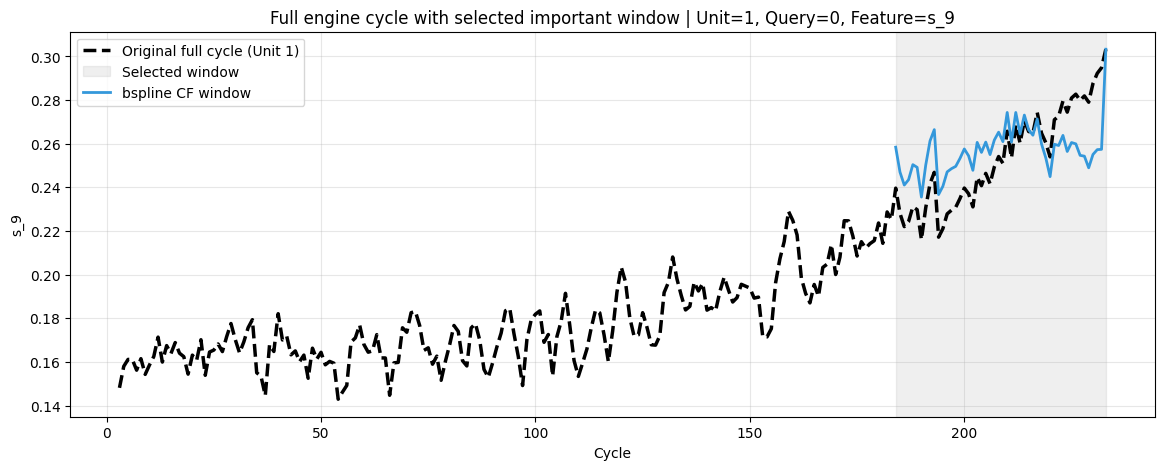
\includegraphics[width=0.9\textwidth]{03_CMAPSS_FD003_latest_Full_engine_cycle.png} \\
		\vspace{0.2cm}
		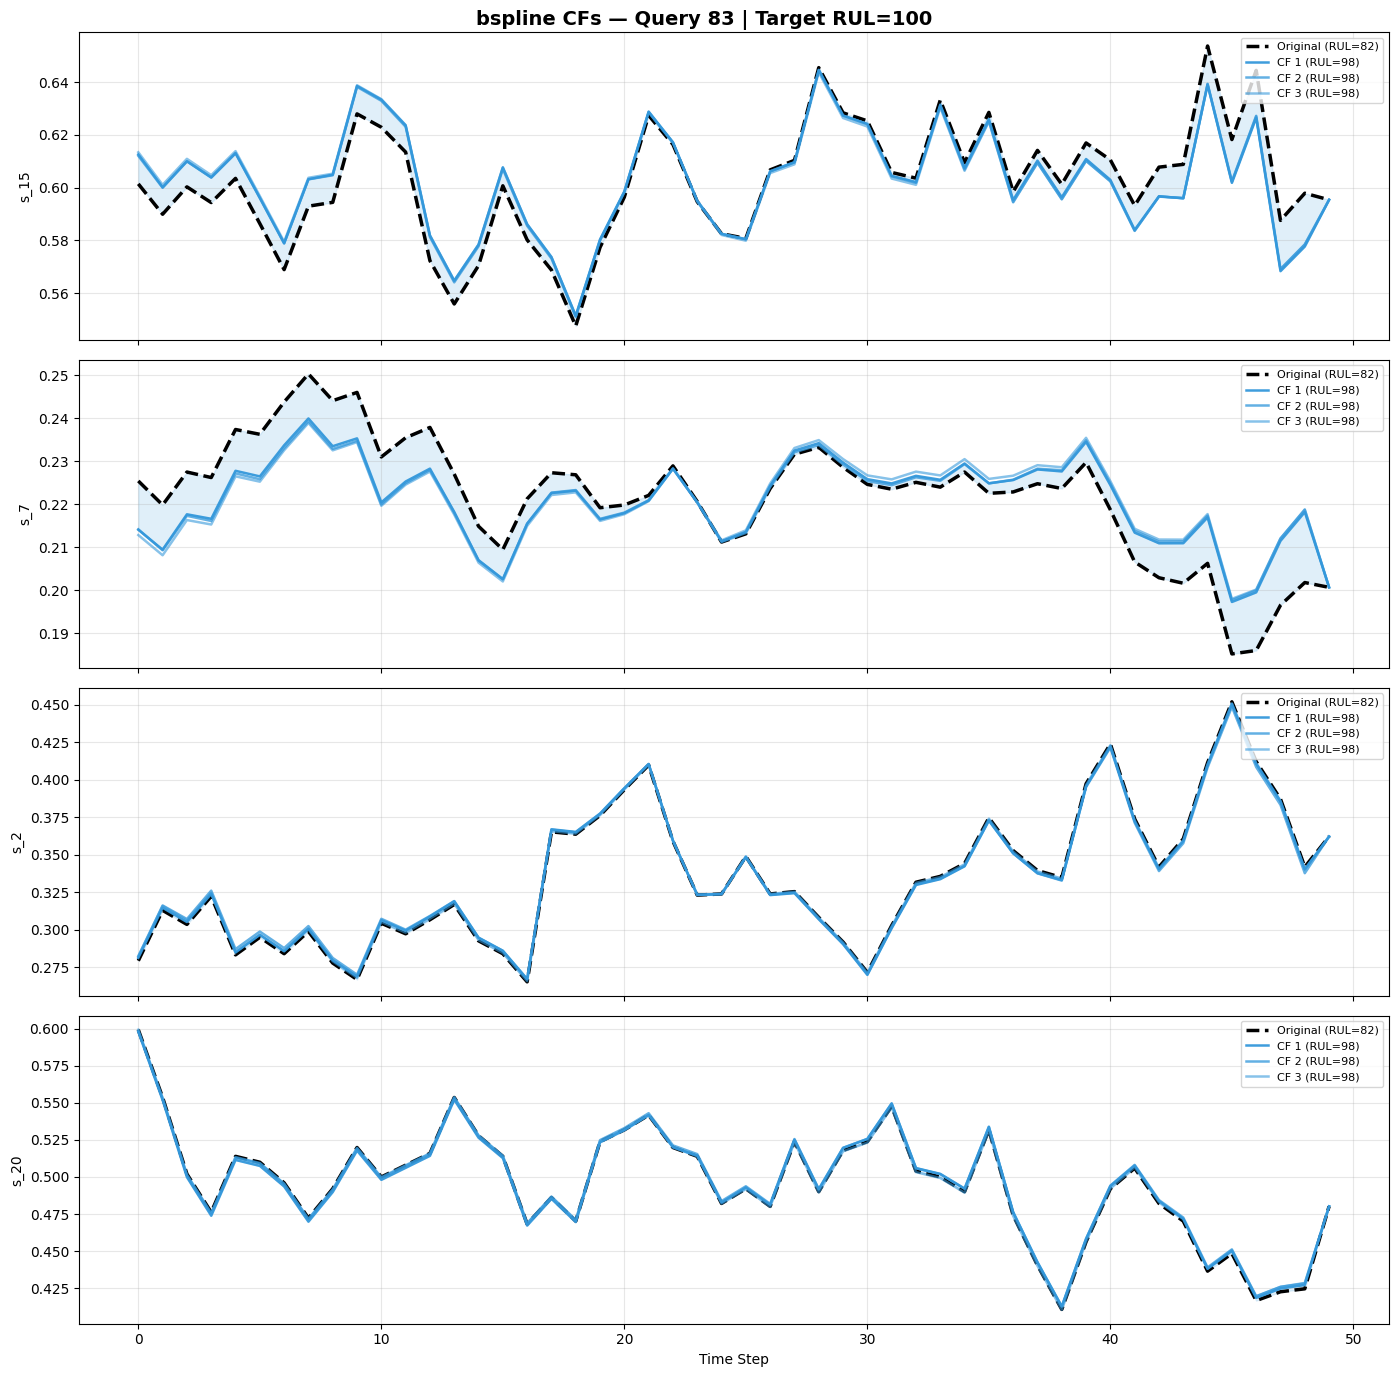
\includegraphics[width=0.9\textwidth]{03_CMAPSS_FD003_latest_Bspline.png}
		\caption{Macroscopic and microscopic evaluation of counterfactual plausibility on CMAPSS FD003. (Top) The B-spline counterfactual is confined to the selected lookback window while following the larger engine-cycle trend. (Bottom) Three smooth counterfactual trajectories for query $83$ move the predicted RUL from $82$ into the target region near $100$.}
		\label{fig:trajectory_macro_micro}
	\end{figure}
	
	\textbf{IEEE Bearing Perturbations.} Figure~\ref{fig:ieee_heatmap} shows the corresponding perturbation footprint for IEEE PRONOSTIA. The B-spline counterfactual remains smooth over the 256-step bearing window and concentrates changes on vibration amplitude and spectral statistics, while mean channels remain nearly unchanged. This provides a qualitative view of the same behaviour observed in Table~\ref{tab:cf_main_results}: the basis space can reach the desired RUL region without introducing scattered point-wise corrections.
	
	\begin{figure}[htbp]
		\centering
		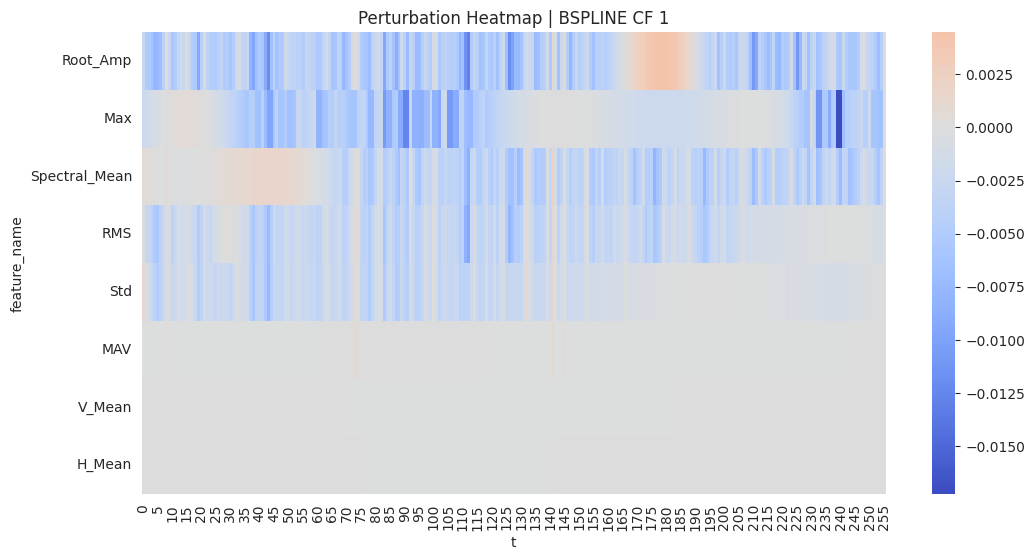
\includegraphics[width=0.7\textwidth]{IEEE.png}
		\caption{IEEE PRONOSTIA perturbation heatmap for a B-spline counterfactual. The edits are smooth over the 256-step bearing window and concentrated on vibration-amplitude and spectral statistics, while mean channels remain nearly unchanged.}
		\label{fig:ieee_heatmap}
	\end{figure}
	
	\textbf{Perturbation Localisation.} Figure~\ref{fig:aep_heatmap} shows the AEP perturbation footprint. The largest magnitude changes occur on the \texttt{Appliances} channel, especially in the later time steps, but the heatmap also contains smaller compensating changes across temperature, humidity, and weather variables. This is expected because the AEP configuration used for this figure allowed state edits. The figure, therefore, illustrates a useful forecasting trade-off: allowing state variables can produce coherent low-energy scenarios, but it is less directly actionable than the action-only setting used for RUL recourse.
	
	\textbf{Validity vs. Proximity.} Figure~\ref{fig:validity_tradeoff} summarises the CMAPSS FD003 trade-off. The basis methods lie on the zero-validity axis, showing that they reach the target band. Among them, RBF and Polynomial are closest to the origin, while Wavelet remains valid but uses a larger perturbation. CoMTE and ForecastCF have small proximity values, but their non-zero validity losses show that the smaller edits often fail to reach the desired RUL region. This supports the main conclusion that the basis space helps the optimiser find target-reaching changes without resorting to temporally jagged corrections.
	
	\begin{figure}[htbp]
		\centering
		\begin{minipage}{0.48\textwidth}
			\centering
			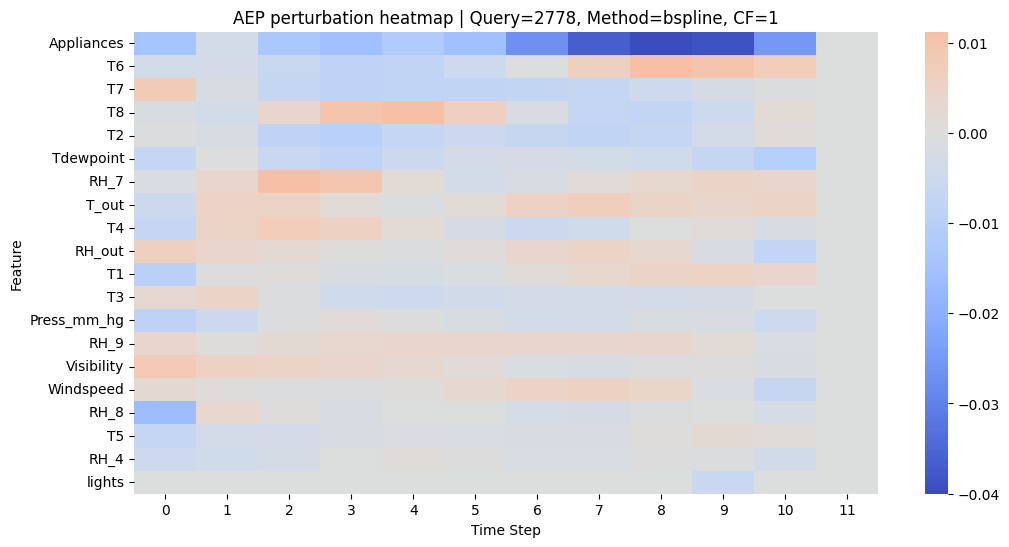
\includegraphics[width=\textwidth]{02_AEP_CF_new_perturbation_heatmap.png}
			\caption{AEP perturbation heatmap for a B-spline counterfactual. The dominant change is on \texttt{Appliances}, with smaller state-feature adjustments due to the editable-state AEP setup.}
			\label{fig:aep_heatmap}
		\end{minipage}\hfill
		\begin{minipage}{0.48\textwidth}
			\centering
			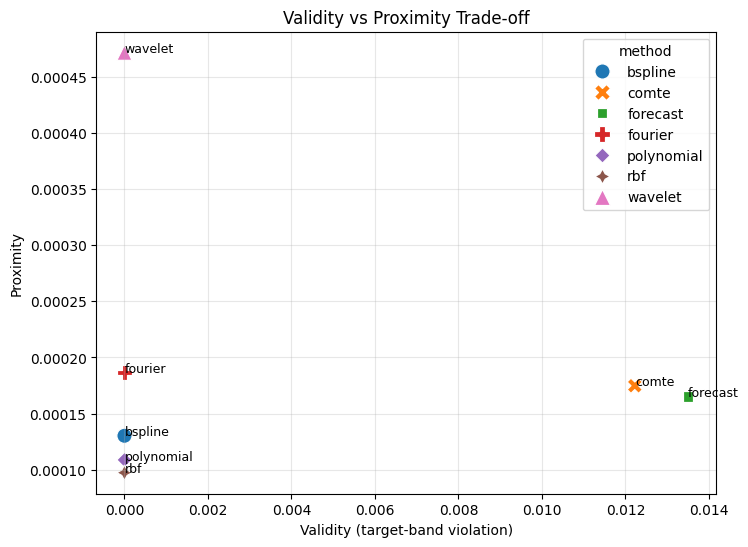
\includegraphics[width=\textwidth]{03_CMAPSS_FD003_latest_validity_vs_proximity.png}
			\caption{Validity--proximity trade-off on CMAPSS FD003. Basis methods reach the target band; RBF and Polynomial provide the most proximal valid solutions.}
			\label{fig:validity_tradeoff}
		\end{minipage}
	\end{figure}
	
	\section{Conclusion}
	In this paper, we introduced a basis-guided framework for generating counterfactual explanations for multivariate time series. By parameterising perturbations in a low-dimensional temporal basis space, the method embeds temporal coherence directly into the optimisation while still balancing validity, proximity, sparsity, smoothness, and diversity. Across NASA CMAPSS, IEEE PRONOSTIA, and AEP, basis-guided counterfactuals usually achieve stronger target validity and group sparsity than point-wise baselines, with the most consistent gains on the RUL tasks.
	
	The main trade-off is computational: basis-space optimisation requires multiple gradient steps and random restarts, but this cost is acceptable in predictive-maintenance and forecasting settings where explanation quality is more important than millisecond inference. A remaining limitation is causal realism: action-only schemas prevent implausible direct edits to state variables, but physical interventions can still produce downstream state changes. Future work will integrate Structural Causal Models (SCMs) into the schema so counterfactuals can simulate such effects rather than only constrain them.
	
	\bibliographystyle{splncs04}
	\bibliography{bibliography/mybibliography}
	
\end{document}